\section{Bound Propagation applied to PyNeVer}
\label{sec:pynever_application}


The PyNeVer algorithm allows for property verification using different levels of refinement. The higher the level of refinement, the more efficient the algorithm becomes. However, as the level of refinement increases, the resulting polytope from the network will be larger than the real one, leading to decreased accuracy in the verification process.\\
Nevertheless, to achieve an exact computation of the output polytope for a given network and property, the minimum level of over-approximation must be used.\\
The objective of this thesis is to leverage bound propagation to improve the efficiency of the PyNeVer algorithm and achieve better time performance. The idea is to utilise bound propagation to determine the node bounds in advance, thereby reducing the number of calculations required during property verification. This will result in a more efficient solution by avoiding redundant computations and focusing only on the regions of interest.

%The GET_BOUNDS function is necessary to understand if a star at which is applied a ReLU function along the j-th dimension must be zeroes along that dimension if it has $ub_j<=0$, or directly propagated if $lb_j>=0$ or must be splitted along the j-th dim if $ub_j >=0 and lw_j<=0$.\\
%The GET_BOUNDS function is function that solves an optimization problem and it is quite expensive. The idea to make more efficient the algorithm is to apply a bound propagation algorithm before running the verification process. In this way it is possible to know a priori which neurons are stable .

\subsection{Real bounds and extimated bounds with bound propagation: all scenarios}
\label{subsec:all_bounds_scenarios}
 The bound propagation performs a calculation that return the numeric bound for all the fully connected layers on the network. Through the upper and lower bound of a neuron we can know if it is stable or unstable. The problem is that the bound propagation implemented must deal with ReLU functions which are not linear and hence introduces an over-approximation.
This implies:
\begin{equation}
	\begin{aligned}
		&lb^* < lb \\
		&ub^* > ub \\
	\end{aligned}
\end{equation}
where $lb$ and $ub$ are the real lower and upper bounds of a node, while $lb*$ and $ub*$ are the overestimated ones.\\
And this over-extimation grows up with the number of ReLU layers.\\
This over-extimation leads to different scenarios:
\begin{itemize}
	\item if the over-extimated lower bound of a node $lb*>0$, knowing that $lb>lb*$ then the neuron is for sure positive stable\\
		\begin{minipage}{\linewidth}
			\centering
			\includegraphics[width=\textwidth]{"Chapter6/img/pos_stable pos_stable"}
		\end{minipage}
	\item if the over-extimated upper bound of a node $ub*<0$, knowing that $ub<ub*$ then the neuron for sure negative stable\\
		\begin{minipage}{\linewidth}
			\centering
			\includegraphics[width=\textwidth]{"Chapter6/img/neg_stable neg_stable"}
		\end{minipage}
	\item if $lb*<0$ and $ub*>0$ knowing that $lb>lb*$ and $ub<ub*$ we cannot state if the neuron is stable or not. We can in turn distinguish three different cases:
	\begin{itemize}
		\item When $lb*<0$ and $lb>0$, in this case the bound propagation suggest that the neuron is unstable while in fact is positive stable\\
			\begin{minipage}{\linewidth}
				\centering
				\includegraphics[width=\textwidth]{"Chapter6/img/unstable pos_stable"}
			\end{minipage}
		\item When $ub*>0$ and $ub<0$, in this case the bound propagation suggests that the neuron is unstable while in fact is negative stable \\
			\begin{minipage}{\linewidth}
				\centering
				\includegraphics[width=\textwidth]{"Chapter6/img/unstable neg_stable"}
			\end{minipage}
		\item When $lb*<0, ub*>0$ and $lb<0, ub>0$, in this case the neuron is unstable as suggested by the bound propagation\\
			\begin{minipage}{\linewidth}
				\centering
				\includegraphics[width=\textwidth]{"Chapter6/img/unstable unstable"}
			\end{minipage}
	\end{itemize}
\end{itemize}
This means that the bound propagation states correctly if a neuron is positive or negative stable. Differently if it states that a neuron is unstable, it isn't possible to get useful information from it.


\subsection{Optimized version of PyNeVer with Bound Propagation}

As discussed earlier, the goal of this thesis is to apply bound propagation to optimize the code of pyNever. As discussed in SubSection \ref{subsec:all_bounds_scenarios}, through the precomputation of bound propagation, given a network and a property, it is possible to identify stable nodes without having to repeatedly call the GET\_BOUNDS function of pyNever. Below, an improved version of pyNever will be presented, which utilizes precalculated bounds to avoid using the GET\_BOUNDS function whenever possible. This enhances the efficiency of the program.

In Section \ref{subsec:all_bounds_scenarios}, we thoroughly examined the concept of bound propagation through precomputation. During this phase, bounds are computed for each node in the network, considering the specified property. The resulting bounds are then stored for later use during program execution.

The enhanced version of pyNever we will present leverages these precalculated bounds to avoid unnecessary calls to the GET\_BOUNDS function. Instead of invoking the function for each star and for each evaluated ReLU node, the program checks if the pre-computated bound states that the node is stable. If so, it is possible to avoid to call the GET\_BOUNDS function. If, differently, the precomputated bound states that the node is unstalbe then it will be necessary to calculate the exact bounds.  This optimization results in a significant improvement in overall performance.

The improved implementation of pyNever introduces an initial phase of bound precomputation, which takes time at program startup but greatly reduces execution time during the evaluation of subsequent nodes. Thanks to this strategy, a part of stable nodes can be efficiently identified without repeating costly computations for each evaluation.

The new version of pyNever, incorporating this improved implementation, offers a substantial advantage in terms of efficiency and execution speed. By minimizing calls to the GET\_BOUNDS function through the use of precalculated bounds, the program can handle large and complex networks more efficiently.

In conclusion, applying bound propagation with precomputed bounds in pyNever represents a significant advancement in code optimization. By utilizing precalculated bounds, the program can rapidly and efficiently identify stable nodes, avoiding redundant calculations and reducing overall execution time. This implementation offers a considerable advantage in the efficiency and usability of pyNever in various application contexts.

\begin{algorithm}[t!]
  \caption{Abstraction of the ReLU activation function with Bound Propagation.}
  \label{alg:new-relu-abst}
  \small
  \begin{algorithmic}[1]
    \Function{compute\_layer}{\emph{input} = $[\Theta_1, \ldots, \Theta_N]$, \emph{refine} = $[r_1, \ldots, r_n]$, \textbf{\emph{lower\_bounds: list}}, \textbf{\emph{upper\_bounds: list}}}
      \State \emph{output} = $[\:]$
      \For{$i = 1:N$} 
        \State \emph{stars} = $[\Theta_i]$
        \For{$j = 1:n$}
          \State \emph{stars} = \textsc{compute\_relu}(\emph{stars}, $j$, \emph{refine}$[j]$, $n$, \textbf{\emph{lower\_bounds[i]}}, \textbf{\emph{upper\_bounds[i]}})
        \EndFor
        \State \textsc{append}(\emph{output}, \emph{stars})
      \EndFor
      \State \Return \emph{output}
    \EndFunction

    \Function{compute\_relu}{\emph{input} = $[\Gamma_1, \ldots, \Gamma_M]$, $j$, \emph{level}, $n$, \textbf{\emph{lower\_bound}}, \textbf{\emph{upper\_bound}}}
      \State $output$ = $[\:]$
      \For{$k = 1:M$}
        \State $is\_positive\_stable$ = False
        \State $is\_negative\_stable$ = False
        \If {$lower\_bound \geq 0$}
          \State $is\_positive\_stable$ = True
        \ElsIf {$upper\_bound \leq 0$}
          \State $is\_negative\_stable$ = True
        \Else
          \State $(lb_j, ub_j)$ = \textsc{get\_bounds}(\emph{input}$[k]$, $j$)
        \EndIf
        \State $M = [e_1\ ...\ e_{j-1}\ 0\ e_{j+1}\ ...\ e_n]$
        \If {$is\_positive\_stable$}
          \State $S$ = \emph{input}$[k]$
        \ElsIf {$is\_negative\_stable$}
          \State $S$ = $M$ * \emph{input}$[k]$
        \ElsIf {$lb_j \geq 0$}
          \State $S$ = \emph{input}$[k]$
        \ElsIf {$ub_j \leq 0$}
          \State $S$ = $M$ * \emph{input}$[k]$
        \Else
          \If{\emph{level} $> 0$}
            \State $\Theta_{low}$ = \emph{input}$[k] \wedge z[j] < 0$;
            $\Theta_{upp}$ = \emph{input}$[k] \wedge z[j] \geq 0$
            \State $S$ = $[M \mbox{ * } \Theta_{low}, \Theta_{upp}]$
          \Else
            \State $(c,V,Cx \leq d)$ = \emph{input}$[j]$
            \State $C_1$ = $[0\ 0\ ...\ -1] \in \mathbb{R}^{1 \times m+1}$, $d_1 = 0$
            \State $C_2$ = $[V[j,:]\ -1] \in \mathbb{R}^{1 \times m+1}$, $d_2 = -c_k[j]$
            \State $C_3$ = $[\frac{-ub_j}{ub_j - lb_j} \cdot V[j,:]\ -1] \in \mathbb{R}^{1 \times m+1}$, $d_3 = \frac{ub_j}{ub_j - lb_j} (c[j] - lb_j)$
            \State $C_0$ = $[C\ 0^{m \times 1}]$, $d_0 = d$
            \State $\hat{C}$ = $[C_0;\ C_1;\ C_2;\ C_3]$, $\hat{d} = [d_0;\ d_1;\ d_2;\ d_3]$
            \State $\hat{V} = MV$, $\hat{V} = [\hat{V}\ e_j]$
            \State $S$ = $(Mc, \hat{V}, \hat{C} \hat{x} \leq \hat{d})$
          \EndIf
        \EndIf
        \State \textsc{append}($output$, $S$)
      \EndFor
      \State \Return $output$
    \EndFunction
  \end{algorithmic}
\end{algorithm}


\subsection{Pynever Complete Verification Example}

\begin{figure}[htbp]
  \centering
  \begin{minipage}[t]{0.4\textwidth}
    	\centering
   	\caption{\label{fig:nn_with_bp} non-bp-case}
	\includegraphics[scale=0.3]{"Chapter6/img/nn_with_bp"}
	\label{fig:nn_with_bp} 
  \end{minipage}
  
  \vspace{1cm}
  
  \begin{minipage}[t]{0.4\textwidth}
   	\centering
   	\caption{\label{fig:nn_without_bp} bp-case}
	\includegraphics[scale=0.3]{"Chapter6/img/nn_without_bp"}
	\label{fig:nn_without_bp}
  \end{minipage}

  \caption{Neural network composed by three FC and two ReLU layers}
  \label{fig:images}
\end{figure}


The Fig~\ref{fig:nn_without_bp} represents a NN composed by:s
\begin{itemize}
	\item Input: the NN has a two dimensional input
	\item FC1: a fully connected layer 2x4
	\item A ReLU activation function is applied to the FC1
	\item FC2: a fully connected layer 4x4 
	\item A ReLU activation function is applied to the FC2
	\item A FC3 4x2. The output is bidimensional
\end{itemize}

%The  FC1 and FC2 layers have the neurons colored in green or red:
%\begin{equation}
%    	\begin{aligned}
%    		& IF neuron color is \textit{green} \mapsto \textit{stable}
%    		& IF neuron color is \textit{red} \mapsto \textit{unstable} 
%    	\end{aligned}
%\end{equation}

In Fig~\ref{fig:nn_without_bp} it is represented a NN without a pre-applied bound propagation. The grey nodes which belongs to the FC layers are nodes whose stability or instability is not knows. Differently, in Fig~\ref{fig:nn_with_bp}, it is pre-applied a bound propagation. It is known a priori if green nodes are positive or negative stable, instead of grey nodes that might be stable or unstable.\\
Below is explained which are the differences and the advantages between the PyNeVer algorithm with bound propagation applied and the "normal" one:
\begin{itemize}
	\item bp-case: PyNeVer algorithm with bound propagation applied
	\item non-bp-case: PyNeVer algorithm without bound propagation applied. 
\end{itemize} 
The PyNeVer algorithm is sequential respect to the layers of the NN, this means that the verification process iterates from the first layer till the last one.
\begin{enumerate}
	\item FC1: the hyper-rectangle star defined by the input property is propagated through the FC1. For PyNeVer algorithm the number of stars in input in a fully connected layer  undergo a transformation (translation or rotation) but don't change in number. In our example we have one star in input in the FC1 layer and so we'll have one star in output. \textbf{The two algorithm versions behave in the same way for FC layers.}
	\item ReLU1:  for computing this layer PyNeVer calls COMPUTE\_LAYER function that, in our example, receives in input 1 star. COMPUTE\_LAYER function calls the function COMPUTE\_RELU one time for each dimension (the $i-th$ ReLU node corresponds to the $i-th$ dimension). \\
\textbf{For both the two algorithms}, the COMPUTE\_RELU bounds is called 4 times. The difference between the two algorithms is that the COMPUTE\_RELU in the non-bp-case must call the GET\_BOUNDS function for all stars along the j-th dimension while in the bp-case the GET\_BOUNDS is called only for the nodes we don't know if they are stable or unstable (the grey ones in fig~\ref{fig:nn_without_bp}). In this case the the bp-case the GET\_BOUNDS function is called 2 times while in the nn-bp-case it is called 4 times.  The max number of output stars is $2^{n_1}$ where $n_1$ is the number of nodes in a generic ReLU layer for each star in input.
	\item FC2: all the input stars undergo a transformation, but the number remains invaried.
	\item ReLU2: the COMPUTER\_LAYER function is called and receives a set of stars as input . For each star is called the COMPUTE\_RELU and for each call are returned at max $2^n_2$ stars. So in the end, the max number of stars returned to COMPUTE\_LAYER function is $2^{n_1}$ * $2^{n_2}$. As for the ReLU1 layer, in the bp-case the GET\_BOUNDS function is not called for stars processed along the dimensions that correspond to the green nodes.
	\item FC3: is the output layer and behaves as the previous fully connected layers.
\end{enumerate}

The GET\_BOUNDS function is necessary to understand if a star at which is applied a ReLU function along the j-th dimension must be zeroes along that dimension if it has $ub_j<=0$, or directly propagated if $lb_j>=0$ or must be splitted along the j-th dim if $ub_j >=0$ and $lw_j<=0$.\\
The GET\_BOUNDS function is function that solves an optimization problem and it is quite expensive. The idea to make more efficient the algorithm is to apply a bound propagation algorithm before running the verification process. In this way it is possible to know a priori which neurons are stable .


%\begin{figure}
%	\centering
%	\caption{\label{fig:over_extimated_bounds} In green the real upper and lower bounds, in red the over-extimated ones}
%	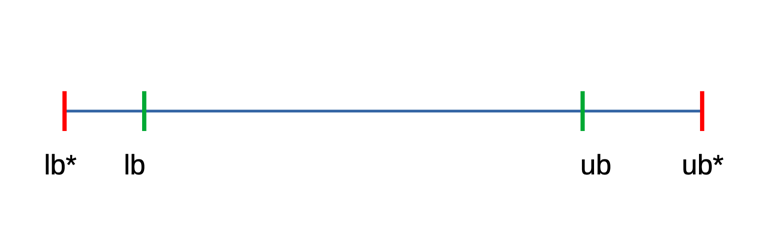
\includegraphics[scale=0.5]{"Chapter6/img/over_extimated_bounds.png"}
%\end{figure}

%\begin{figure}[htbp]
%  \centering
%  \begin{minipage}[b]{0.4\textwidth}
%    \centering
%    \includegraphics[width=\textwidth]{"Chapter6/img/neg_stable neg_stable"}
%    \caption{Prima immagine}
%    \label{fig:img1}
%  \end{minipage}
%  \hfill
%  \begin{minipage}[b]{0.4\textwidth}
%    \centering
%    \includegraphics[width=\textwidth]{"Chapter6/img/neg_stable neg_stable"}
%    \caption{Seconda immagine}
%    \label{fig:img2}
%  \end{minipage}
%\end{figure}

\subsection{Bound Propagation Pseudocode}
\begin{algorithm}[t!]
  \caption{Bound Propagation Algorithm}
  \label{alg:bp-pseudocode}
  \small
\begin{algorithmic}[1]
	\Function{ComputeBounds}{\emph{network}, \emph{property}}
    		\State \Comment{the PropertyFormatConverter takes in input a PyNeVer property and return and return an HyperRectangleBounds}
   		 \State $property\_converter = {PropertyFormatConverter}(\text{property})$
    
    		\State $input\_hyper\_rect = property\_converter.get\_vectors()$
    
    		\State $layers = \text{get\_abstract\_network}(\text{network})$
    
   		\State $input\_size = input\_hyper\_rect.get\_size()$
    
    		\State $lower = \text{LinearFunctions}(\text{np.identity(input\_size)}, \text{np.zeros(input\_size)})$
    
    		\State $upper = \text{LinearFunctions}(\text{np.identity(input\_size)}, \text{np.zeros(input\_size)})$
    
    		\State $input\_bounds = \text{SymbolicLinearBounds}(lower, upper)$
    
    		\State $numeric\_preactivation\_bounds = \text{dict}()$
    
   		\State $numeric\_postactivation\_bounds = \text{OrderedDict}()$
    
    		\State $symbolic\_bounds = \text{dict}()$
    
    		\State $current\_input\_bounds = input\_bounds$
    
    		\For{$i$ \textbf{in} $0$ \textbf{to} $\text{len}(layers) - 1$}
    
       			\If{$layers[i]$ \text{ is instance of } $\text{ReLU}$}
            			\State $symbolic\_activation\_output\_bounds = \text{compute\_relu\_output\_bounds}(symbolic\_dense\_output\_bounds, input\_hyper\_rect)$
            
            			\State $postactivation\_bounds = \text{HyperRectangleBounds}(\text{np.maximum}(preactivation\_bounds.\text{get\_lower}(), 0), 							\text{np.maximum}(preactivation\_bounds.\text{get\_upper}(), 0))$
            
       			\ElsIf{$layers[i]$ \text{ is instance of } $\text{FullyConnected}$}
            			\State $symbolic\_dense\_output\_bounds = \text{compute\_dense\_output\_bounds}(layers[i], current\_input\_bounds)$
            
            			\State $preactivation\_bounds = symbolic\_dense\_output\_bounds.\text{to\_hyper\_rectangle\_bounds}(input\_hyper\_rect)$
            
            			\State $symbolic\_activation\_output\_bounds = symbolic\_dense\_output\_bounds$
            
            			\State $postactivation\_bounds = \text{HyperRectangleBounds}(preactivation\_bounds.\text{get\_lower}(), preactivation\_bounds.\text{get\_upper}())$
            
        				\Else
            				\State \textbf{raise} \text{Exception}            
        			\EndIf
        
        			\State $symbolic\_bounds[layers[i].\text{identifier}] = (symbolic\_dense\_output\_bounds, symbolic\_activation\_output\_bounds)$
        
        			\State $numeric\_preactivation\_bounds[layers[i].\text{identifier}] = preactivation\_bounds$
        
        			\State $numeric\_postactivation\_bounds[layers[i].\text{identifier}] = postactivation\_bounds$
        
        			\State $current\_input\_bounds = symbolic\_activation\_output\_bounds$
        
    		\EndFor
    
    		\State \textbf{return} $numeric\_postactivation\_bounds$
    
	\EndFunction
\end{algorithmic}
\end{algorithm}

\begin{algorithm}
\caption{Class HyperRectangleBounds}
\label{alg:hyper-rect-bound}
\begin{algorithmic}[1]
\Procedure{HyperRectangleBounds}{}
    \State \textbf{public} $lower: list$
    \State \textbf{public} $upper: list$
\EndProcedure

\Procedure{Constructor}{}
    \State $lower = $ initialize
    \State $upper = $ initialize
\EndProcedure

\end{algorithmic}
\end{algorithm}



